\chapter{Simulace}
\label{chap:sim}

Jak již bylo zmíněno v předchozí kapitole a jak vychází z názvu této práce, značnou částí našeho zkoumání bylo také počítačové simulování těchto systémů.

\section{Popis způsobu simulování}

Naším cílem bude vytvoření tzv. \textit{"Discrete event simulation"} neboli \textit{DES} \cite{sim_methods}. Jedná se o druh simulační metody, která popisuje náš stav pomocí diskrétních stavů, které existují v daném čase. Z jednoho určitého stavu poté pomocí určitých pravidel popisujících náš systém simulační algoritmus provádí odhad toho, jak bude vypadat další stav po uplynutí $\Delta t$ sekund, kde $\Delta t$ je velmi malé. Toto nazveme nejdím simulačním krokem. Poté stačí opakovat simulační kroky dle libosti.

\subsection{Runge-Kutta metody}

Runge-Kutta metody, pojmenované po Carlu Davidu Tolmé Rungeovi a Martinu Wilhelmu Kuttovi, jsou rodinou metod používaných k řešení implicitních a explicitních diferenciálních rovnic. Implicitní metody popisující budoucí stav systému z předchozího stavu, stejně jak budeme dělat my v naší \textit{DES}. Runge-Kutta metody (také ornačované pouze RK metody) jsou tedy ideálním nástrojem pro simulování našeho problému. nejjednodušším příkladem RK metody je například Eulerova metoda. Těchto metod je nespočet, ale jejich obecný předpis je následující \cite{RK_def}:
\begin{equation}
    \label{eq:RK_def}
    \begin{gathered}
        y_{n+1} = y_n + \Delta t \sum_{i=1}^{s} b_i k_i \\
        k_m = f \Bigg(t_n + c_m \Delta t, y_n + \Bigg(\sum_{j=1}^{s-1} k_j a_{m,j} \Bigg) \Delta t \Bigg)
    \end{gathered}
\end{equation}

V tomto předpisu jednotlivé znamenají: $t_n$ je čas stavu $y_n$ a $\Delta t$ je krátký časový krok; $s$ je stupeň RK metody; $a_{m,j}$, $b_i$ a $c_m$ jsou specifické koeficinty dané RK metody; $y_n$ je stávající stav a $y_{n+1}$ je budoucí, předpovídaný, stav; $k_m$ je pomocný sub-stav; $f(t,y) = \dot{y}$.

Specifick0 koeficienty se nejčastěji zapisují pomocí tzv. Butcherových tabulek \cite{Butcher_tab_def} (pojmenovaných po Johnu Charlesovi Butcherovi). Zápis obecné Butcherovy tabulky pro RK metodu $s$. stupně je:
\begin{table}[!ht]
    \centering
    \captionsetup{singlelinecheck=off}
    \caption{Zápis obecné Butcherovy tabulky pro RK metodu $s$. stupně}
    \label{tab:Butch_tab}

    \begin{tabularx}{7cm}{c | c c c c c}
        $c_1 = 0$                                                            \\
        $c_2$    & $a_{2, 1}$                                                \\
        $c_3$    & $a_{3, 1}$ & $a_{3, 2}$                                   \\
        $\vdots$ & $\vdots$   &            & $\ddots$                        \\
        $c_s$    & $a_{s, 1}$ & $a_{s, 2}$ & $\cdots$ & $a_{s, s-1}$         \\
        \hline
                 & $b_1$      & $b_2$      & $\cdots$ & $b_{s-1}$    & $b_s$ \\
    \end{tabularx}
\end{table}

Některé z podmínek, které sice nezaručují konzistentnost a stabilitu metody, ale dobrými základními pravidly jsou \cite{Butcher_tab_def}:

\begin{equation}
    \label{eq:RK_conditions}
    \begin{gathered}
        \text{1)} \quad \quad \qquad \qquad \sum_{i=1}^{s} b_i = 1 \qquad \qquad \\
        \text{2)} \quad \quad \sum_{j=1}^{i-1} a_{i,j} = c_i \quad (i \in \{2,...,s\})
    \end{gathered}
\end{equation}

Níže vypíšeme Butcherovy tabulky několika základních metod, které byly později implementovány v simulaci \cite{RK_methods_list}:

\begin{table}[H]
    \parbox{.45\linewidth}{
        \centering
        \caption[Butcherova tabulka Eulerovy metody]{\textbf{Eulerova metoda}}
        \begin{tabular}{c | c}
            0 &   \\
            \hline
              & 1 \\
        \end{tabular}
    }
    \hfill
    \parbox{.45\linewidth}{
        \centering
        \caption[Butcherova tabulka metody středního bodu]{Metoda středního bodu}
        \begin{tabular}{c | c c}
            0   &         \\
            1/2 & 1/2     \\
            \hline
                & 0   & 1 \\
        \end{tabular}
    }
\end{table}
\begin{table}[H]
    \parbox{.3\linewidth}{
        \centering
        \caption[Butcherova tabulka Heunovy metody]{Heunova metoda}
        \begin{tabular}{c | c c}
            0 &           \\
            1 & 1         \\
            \hline
              & 1/2 & 1/2 \\
        \end{tabular}
    }
    \hfill
    \parbox{.3\linewidth}{
        \centering
        \caption[Butcherova tabulka Ralstonovy metody]{Ralstonova metoda}
        \begin{tabular}{c | c c}
            0   &           \\
            2/3 & 2/3       \\
            \hline
                & 1/4 & 3/4 \\
        \end{tabular}
    }
    \hfill
    \parbox{.3\linewidth}{
        \centering
        \caption[Butcherova tabulka obecné metody 2. stupně]{Obecná metoda 2. stupně}
        \begin{tabular}{c | c c}
            0        &                                               \\
            $\alpha$ & $\alpha$                                      \\
            \hline
                     & $1 - \frac{1}{2\alpha}$ & $\frac{1}{2\alpha}$ \\
        \end{tabular}
    }
\end{table}

\begin{table}[H]
    \parbox{.45\linewidth}{
        \centering
        \caption[Butcherova tabulka Simpsonova pravidla 3/8]{Simpsonovo pravidlo 3/8}
        \begin{tabular}{c | c c c c c}
            0   &                        \\
            1/3 & 1/3                    \\
            2/3 & -1/3 & 1               \\
            1   & 1    & -1  & 1         \\
            \hline
                & 1/8  & 3/8 & 3/8 & 1/8 \\
        \end{tabular}
    }
    \hfill
    \parbox{.45\linewidth}{
        \centering
        \caption[Butcherova tabulka RK4]{\textbf{Standardní Runge-Kutta metoda 4. stupně (neboli RK4)}}
        \begin{tabular}{c | c c c c c}
            0   &                       \\
            1/2 & 1/2                   \\
            1/2 & 0   & 1/2             \\
            1   & 0   & 0   & 1         \\
            \hline
                & 1/6 & 2/6 & 2/6 & 1/6 \\
        \end{tabular}
    }
\end{table}

\begin{table}[H]
    \hfill
    \parbox{.8\linewidth}{
        \centering
        \caption[Butcherova tabulka Ralstonovy metody 4. stupně]{Ralstonova metoda 4. stupně}
        \begin{tabular}{c | c c c c c}
            0          &                                                    \\
            0.4        & 0.4                                                \\
            0.45573725 & 0.29697761 & 0.15875964                            \\
            1          & 0.21810040 & -3.05096516 & 3.83286476              \\
            \hline
                       & 0.17476028 & -0.55148066 & 1.20553560 & 0.17118478 \\
        \end{tabular}
    }
    \hfill
\end{table}

\section{Popisující interakce}
Řídícími interakcemi našeho simulovaného modelu budou opět popsány rovnicemi \ref{eq:F_m} a \ref{eq:B}. V simulaci se však zaměříme na interakce celých spinnerů, ne pouze 2 dipólů. Pro popsání spinneru musíme určit několik vlastností týkajících se:
\begin{enumerate}[topsep=0pt, partopsep=0pt]
    \setlength{\itemsep}{0pt}%
    \setlength{\parskip}{0pt}%
    \item \textbf{Konfigurace}: pozice, velikosti, počet ramen (viz \autoref{sub:param_konf})
    \item \textbf{Pohybu}: úhlová rychlost, moment setrvačnosti (viz \autoref{sec:moment_of_inertia}), třecí koeficienty (viz \autoref{chap:drag})
    \item \textbf{Magnetů}: velikost momentů, remanence (viz \autoref{sec:remanence_measurement}), orientace (viz \autoref{fig:mag_orientations})
\end{enumerate}

Naším cílem je popisovat rotaci jednotlivých spinnerů v čase. Toto provedeme určením celkového momentu sílu jakožto součtu silových a magnetických složek přes všechny externí magnetické momenty. Popisující rovnice spinneru jsou tedy \footnote{První rovnice vychází z definice momentu síly: $\dot{L} = I \dot{\omega} = \tau$}:
\begin{equation}
    \label{eq:sim_equations}
    \begin{gathered}
        I\dot{\omega} = \sum_{external} (\tau_F + \tau_{mag}) \\
        \dot{\varphi} = \omega \\
    \end{gathered}
\end{equation}

Ve výše uvedených rovnicí $\tau_F$ popisuje moment síly pocházející ze silové interakce, kterým na spinner (neboli na všechny jeho magnety) působí nějaký externí magnetický moment $m_{external}$ umístěný v prostoru na pozici $P_{external}$. Moment síly určíme pomocí ramene $r$, přes které síla $F$ na spinner působí: $\vec{\tau} = \vec{F} \times \vec{r}$.

$\tau_{mag}$ popisuje moment síly pocházející z toho, že na každý magnet spinneru působí externí magnetické pole $B(r, m_{external})$ tvořené externím magnetickým momentem $m_{external}$ umístěný v prostoru na pozici $P_{external}$. Pomocí momentu magentu umístěného na spinneru jednoduše dopočítáme moment síly podle rovnice \ref{eq:B}: $\tau = m \times B(r, m_{external})$.

Předpisy $\tau_F$ a $\tau_{mag}$ jsou:
\begin{equation}
    \label{eq:sim_equations2}
    \begin{gathered}
        \tau_F = \sum_{j=0}^{n} F_m(P_{external}- P(j), m(j), m_{external}) \times (P(j) - S)\\
        \tau_{mag} = \sum_{j=0}^{n} m(j) \times B(P(j)-P_{external},m_{external})\\
    \end{gathered}
\end{equation}

\section{Implementace}
K implementaci naší simulace použijeme sotwarový systém zvaný \texttt{Node.js}, který používá programovací jazyk \texttt{JavaScript (JS)} \cite{JS}. K tomuto rozhodnutí jsme došli, jelikož \texttt{Node.js} je rychlejší než \texttt{Python}, ale stále nabízí větší množství programátorsky nápomocných prvků. Pro nás to bude ideální kompromis mezi jednoduchostí implementace a rychlostí. V průběhu implementace také používáme datového formátu \texttt{JSON} \cite{JSON} a nativní knihovnu \texttt{Node.js} zvanou \texttt{fs (File System)}, pomocí které budeme naše výsledky exportovat do \texttt{.csv} souborů pro další zpracování. Použití jazyka \texttt{JavaScript} také nabízí jednoduché znovupoužití již napsaného kódu k vytvoření webového rozhraní s vizualizací simulovaného systému. Toto rozhraní je skvělé k odstraňování chyb v průběhu vývoje a zároveň zjednodušuje interpretaci generovaných výsledků.

\subsection{Použité datové struktury}

\subsubsection{3D vektory}

První datovou strukturou, kterou budeme používat v našich výpočtech jsou 3D vektory. Jejich implementace společně s užitečnými funkcemi (sčítání, odčítání, vektorov a skalární násobení, apod.) je triviální.

3D vektory v našem kódu budou instancí třídy pojmenované \textbf{\texttt{v3}} a jejich jediné vlastnosti jsou jejich $x,y$ a $z$ komponenty vyjádřené jako 64-bitová čísla podle standardu \texttt{IEEE 754} \cite{IEEE-754}.

\subsubsection{Spinnery}

Další strukturou jsou jednotlivé spinnery, které budeme označovat symbolem $\mathbb{S}$ a případně odpovídajícím číselným indexem, či jiným identifikátorem v pravém dolním indexu. Je-li z kontextu zřejmé, o jaký spinner se jedná, můžeme k jeho vlastnosnostem referovat čistě podle znaků určených v nomenklatuře (viz \autoref{sec:nomenclature}). Je-li potřeba oddělovat jednotlivé spinnery, budeme k jejich vlastnostem referovat exaktně a to skrze horní index; například, chtěli bychom-li určit počet ramen (značeno písmenem $n$) nějakého externího spinneru, použili bychom $\mathbb{S}_{external}^{n}$. Pokud bychom chtěli získat pozici 1. magnetu 3. spinneru, použili bychom $\mathbb{S}_{3}^{P}(1)$, jelikož $P(i)$ je funkce. Pomocí tohoto způsobu zápisu také v průběhu následujících kapitol konkretizujeme rovnice \ref{eq:sim_equations} a \ref{eq:sim_equations2}.

V kódu jsou spinnery instancí třídy \textbf{\texttt{spinner}}, jejíž vlastnosti jsou vypsány v tabulce \ref{tab:sim_spinner_properties}.

\DFNalwaysdouble
\DFNallowcbreak
\DFNcolumnwidth 0.475\textwidth
\begin{table}[!ht]
    \captionsetup{justification=raggedright,singlelinecheck=off}
    \caption[Výpis vlastností třídy \textbf{\texttt{spinner}}]{Výpis vlastností třídy \textbf{\texttt{spinner}}:}
    \label{tab:sim_spinner_properties}

    \begin{tabular}{p{0.275\textwidth} p{0.45\textwidth} p{0.275\textwidth} }
        \textbf{Symbol}                                                                                                                 & \textbf{Datový typ}                                   & \textbf{Iniciální hodnota}                                 \\
        \hline
        $r$                          \tablefootnote{Poloměr (viz \autoref{fig:spinner_size})}                                           & \texttt{float64}                                      & 0.0359                                                     \\
        $S$                          \tablefootnote{Střed}                                                                              & \texttt{v3}                                           & žádná                                                      \\
        $I$                          \tablefootnote{Moment setrvačnosti (viz \autoref{sec:moment_of_inertia})}                          & \texttt{float64}                                      & $4.80 \cdot 10^{-5}$                                       \\
        $\varphi_0$                  \tablefootnote{Počáteční úhel}                                                                     & \texttt{float64}                                      & žádná                                                      \\
        $\varphi$                    \tablefootnote{Okamžitý úhel}                                                                      & \texttt{float64}                                      & žádná                                                      \\
        $\omega_0$                   \tablefootnote{Počáteční úhlová rychlost}                                                          & \texttt{float64}                                      & žádná                                                      \\
        $\omega$                     \tablefootnote{Okamžitý úhlová rychlost}                                                           & \texttt{float64}                                      & žádná                                                      \\
        $\alpha$                     \tablefootnote{Konstantní koeficient tření (viz \autoref{chap:drag})}                              & \texttt{float64}                                      & 0.868                                                      \\
        $\beta$                      \tablefootnote{Lineární koeficient tření (viz \autoref{chap:drag})}                                & \texttt{float64}                                      & 0.0                                                        \\
        $\gamma$                     \tablefootnote{Kvadratický koeficient tření (viz \autoref{chap:drag})}                             & \texttt{float64}                                      & 0.00068                                                    \\
        $n$                          \tablefootnote{Počet ramen/magnetů}                                                                & \texttt{int}                                          & 3                                                          \\
        $m_0$                        \tablefootnote{Velikost magnetického momentu (viz \autoref{eq:mag_mom_remanence})}                 & \texttt{float64}                                      & $\frac{1.1049 \cdot 0.005^3}{4\pi \cdot 10^{-7}} = 0.1099$ \\
        \texttt{magnet\_orientation} \tablefootnote{Orientace magnetů (viz \autoref{fig:mag_orientations})}                             & \texttt{"vertical" / "radial" / "tangent"}            & \texttt{"vertical"}                                        \\
        \texttt{constant\_}$\omega$  \tablefootnote{Určuje, zda má úhlová rychlost spinneru zůstat konstantní (simuluje hnaný spinner)} & \texttt{bool}                                         & false                                                      \\
        $m(i)$                       \tablefootnote{Funkce vracející orientaci magnetu podle jeho indexu}                               & \texttt{funkce (int $\rightarrow$ v3)}                & nelze měnit                                                \\
        $P(i)$                       \tablefootnote{Funkce vracející pozici magnetu podle jeho indexu}                                  & \texttt{funkce (int $\rightarrow$ v3)}                & nelze měnit                                                \\
        \texttt{copy ()}             \tablefootnote{Funkce vracející novou instanci spinneru se stejným stavem}                         & \texttt{funkce ($\varnothing$ $\rightarrow$ spinner)} & nelze měnit
    \end{tabular}
\end{table}

\clearpage

\DFNtrysingle
\DFNinhibitcbreak
\DFNcolumnwidth 1\textwidth

\subsubsection{$\Omega$-stavy}

Další důležitou datovou strukturou je něco, co nazveme $\Omega$-stav. Tato datová struktura má za úkol uložit celkový stav systému (tedy stavy všech spinnerů - řekněme, že jejich počet bude $p$) a provádět na nich operace potřebné k řešení diferenciálních rovnic pomocí RK metod. Druhým úkolem $\Omega$-stavů je výpočet všech momentů sil pro všechny spinnery - toto v popisu RK metody (viz \autoref{eq:RK_def}) představuje naši derivaci, neboli funkci $f$.

Hlavní vlastností $\Omega$-stavů je tedy pole spinnerů označované $\mathbb{P} = \{ \mathbb{S}_1, \mathbb{S}_2, \ldotp ,\mathbb{S}_p \}$ o velikoti $|\Omega_{}^{\mathbb{P}}| = \Omega_{}^{p}$. Na obecný $k$. prvek tohoto pole se budeme odkazovat následovně: $\Omega_{}^{\mathbb{P}}(k) = \mathbb{S}_k$.

Jelikož úkolem $\Omega$-stavu je i určení všech momentů sil, bude mít i vlastnost značenou $A$, což je pole dopočítaných úhlových zrychlení jednotlivých spinnerů. Pole $A$ tedy ukládá všechna vypočtená úhlová zrychlení všech spinnerů, která získáme z rovnice \ref{eq:sim_equations}. Jednotlivá zrychlení označíme symbolem $\alpha$ a tím pádem $A = \{ \alpha_1, \alpha_2, \ldotp, \alpha_p \} $. Na jednotlivé prvky se opět odkazujeme takto: $\Omega_{}^{A}(k) = \alpha_k = \dfrac{\mathbb{S}_k^\tau}{\mathbb{S}_k^I}$.

Nyní je na řadě provést formalizaci řídících rovnic \ref{eq:sim_equations} a \ref{eq:sim_equations2} pomocí tohoto způsobu zápisu. Začneme rovnicemi pro výpočet silové a magnetické interakce magnetů, které nyní popíšeme jakožto funkce tří parametrů. Prvním parametrem v pořadí bude spinner $\mathbb{S}$, pro který budeme počítat momenty sil, kterými na něj působí externí magnetický moment $m_{external}$ nacházející se na pozici $P_{external}$:
\begin{equation}
    \label{eq:sim_equations_formalized}
    \begin{gathered}
        \ \\
        \overbrace{
            \tau_F (\mathbb{S}, m_{external}, P_{external})
        }^{\mathclap{\substack{\text{Moment síly z} \\
                \text{silové interakce}}}}
        =
        \underbrace{
        \sum_{j=1}^{\mathbb{S}^{n}}
        }_{\mathclap{\text{Iterace přes všechny magnety spinneru}}}
        \overbrace{
            F_m(P_{external} - \mathbb{S}^{P}(j), \mathbb{S}^{m}(j), m_{external})
        }^{\mathclap{\substack{\text{Síla mezi $j$. magnetem spinneru} \\
                    \text{ a externím magnetickým momentem}}}}
        \times
        \underbrace{
            (\mathbb{S}^{P}(j) -  \mathbb{S}^{S})
        }_{\mathclap{\text{Rameno síly}}} \\
        \ \\
        \overbrace{
            \tau_{mag}(\mathbb{S}, m_{external}, P_{external})
        }^{\mathclap{\substack{\text{Moment síly z} \\
                \text{magnetické interakce}}}}
        =
        \underbrace{
        \sum_{j=1}^{\mathbb{S}^{n}}
        }_{\mathclap{\text{Iterace přes všechny magnety spinneru}}}
        \mathbb{S}^{m}(j)
        \times
        \overbrace{
        B(\mathbb{S}^{P}(j)-P_{external},m_{external})
        }^{\mathclap{\substack{\text{Magnetické pole tvořené externím} \\
                \text{momentem na pozici $j.$ magnetu}}}} \\
    \end{gathered}
\end{equation}

\clearpage

Nyní, když jsme formalizovali silové a magnetické interakce z jednoho externího magnetického dipólu, stačí určit celkový moment síly $\tau_{tot}$, kterým na spinner působí všechny magnety dohromady.
$\tau_{tot}$ tedy bude součet obou složek ze všech magnetů všech ostatních spinnerů.
Jako poslední také nesmíme zapomenou na započítání třecích účinků spinneru.
Z $\tau_{tot}$ konečně dopočítám úhlové zrychlení $\alpha_k$ obecného $k$. spinneru $\mathbb{S}_k$ takto:
\begin{equation}
    \label{eq:sim_equations_formalized2}
    \begin{gathered}
        \alpha_k = \frac{\tau_{tot}}{I} =
        \frac{1}{\mathbb{S}_k^I}
        \Bigg(
        \underbrace{
        \sum_{j=1; j \neq k}^{|\Omega^{\mathbb{P}}|}
        }_{\mathclap{\substack{\text{Iterace přes všechny} \\
                \text{ostatní spinnery $\mathbb{S}_j$}}}}
        \overbrace{
        \sum_{i=1}^{\mathbb{S}_j^n}
        }^{\mathclap{\substack{\text{Iterace přes všechny} \\
                \text{magnety spinneru $\mathbb{S}_j$}}}}
        \bigg(
        \underbrace{
            \tau_F (\mathbb{S}_k, \mathbb{S}_j^m (i), \mathbb{S}_j^P (i))
        }_{\mathclap{\text{Silová složka}}}
        +
        \underbrace{
        \tau_{mag} (\mathbb{S}_k, \mathbb{S}_j^m (i), \mathbb{S}_j^P (i))
        }_{\mathclap{\text{Magnetická složka}}}
        \bigg)
        -
        \\
        \qquad
        \qquad
        \qquad
        \qquad
        \qquad
        \qquad
        -
        \underbrace{
        \bigg( 
        \mathbb{S}_k^{\alpha}
        + \mathbb{S}_k^{\beta} \cdot \mathbb{S}_k^{\omega} 
        + \mathbb{S}_k^{\gamma} \cdot (\mathbb{S}_k^{\omega})^2
        \bigg)
        }_{\mathclap{\text{Třecí složka}}}
        \Bigg)
    \end{gathered}
\end{equation}

Pro další výpočty ještě zavedeme, jak se chová sčítání stavů a násobení $\Omega^A$ časem.
Jednoduše řečeno dochází k sčítání hodnot pro každý index, nebo k násobení hodnoty na každém indexu daným časem\footnote{V rovnici \ref{eq:sim_equations_formalized4} jsou jednotky: $[rad \cdot s^{-1}] = [rad \cdot s^{-2}] \cdot [s]$.}.
Matematicky bychom tedy tyto operace formulovali takto\footnote{Podmínkou sčítání je, že: $\Omega_{sum}^p = \Omega_{a}^p = \Omega_{b}^p$}:

\begin{equation}
    \label{eq:sim_equations_formalized3}
    \begin{gathered}
        \text{Sčítání: }\quad
        \Omega_{sum} = \Omega_{a} + \Omega_{b} \\
        \Updownarrow \\
        \Omega_{sum}^{\mathbb{P}}(k)^{\omega} = \Omega_{a}^{\mathbb{P}}(k)^{\omega} + \Omega_{b}^{\mathbb{P}}(k)^{\omega}
        \quad \forall k \in {1, \ldots, \Omega^{p}} \\
    \end{gathered}
\end{equation}

\begin{equation}
    \label{eq:sim_equations_formalized4}
    \begin{gathered}
        \text{Násobení:}\quad
        \Omega_{b} = \Omega_{a}^A \cdot t \quad \quad \\
        \Updownarrow \\
        \Omega_{b}^{\mathbb{P}}(k)^{\omega} = \Omega_{a}^{A}(k) \cdot t
        \quad \forall k \in {1, \ldots, \Omega^{p}} \\
    \end{gathered}
\end{equation}

S tímto jsme konečně schopni definovat poslední vlastnost $\Omega$-stavu, kterou je krátky časový úsek $\delta$.
Z výpočtu zrychlení je pak provedena predikce budoucího stavu pod uplynutí $\delta$, který označíme $\prescript{*}{}\Omega$.
Jeho definicí je:

\begin{equation}
    \label{eq:sim_equations_formalized5}
    \begin{gathered}
        \prescript{*}{}{\Omega} = \Omega + \Omega^A \cdot \Omega^{\delta}
    \end{gathered}
\end{equation}

V kódu jsou tyto struktury instancemi třídy \texttt{omega\_state}.

\clearpage

\subsubsection{$\Phi$-stavy}

Poslední datovou strukturou jsou tzv. $\Phi$-stavy, které jsou velmi podobné $\Omega$-stavům svou funkcí. Jejich účelem je opět umožnit použití RK metod. V průběhu jednoho simulačního kroku totiž dochází k dvojitému numerickému integrování - nejdříve, abychom získali z úhlového zrychlení úhlovou rychlost, a poté podruhé, abychom z úhlové rychlosti získali úhel
($\alpha_k \xRightarrow{RK} \mathbb{S}_k^{\omega}  \xRightarrow{RK} \mathbb{S}_k^{\varphi}$).

Vlastnosti $\Phi$-stavů jsou stejné jako u $\Omega$-stavů, kromě pole $A$, které je nahrazeno polem $O$. Pole $O$, narozdíl od pole $A$, které ukládá úhlová zrychlení, obsahuje úhlové rychlosti každého spinneru. Pole $O$ zapisujeme takto: $\Phi{}^{O} = \{ \omega_1, \omega_2, \ldots, \omega_p\}$. Na libovoný $k$. člen se opět odkazujeme takto: $\Phi{}^{O}(k) = \omega_k$. $\Omega$-stavy a $\Phi$-stavy na sebe navazují následovně:

\begin{equation}
    \label{eq:sim_equations_formalized6}
    \begin{gathered}
        \Phi^O(k) = {\Omega}^{\mathbb{P}}(k)^{\omega}
        \quad
        \forall k \in {1, \ldots, \Phi^{p}} \\
    \end{gathered}
\end{equation}

Poté je predikce dalšího $\Phi$-stavu analogická predikci $\Omega$-stavu:

\begin{equation}
    \label{eq:sim_equations_formalized7}
    \begin{gathered}
        \prescript{*}{}{\Phi} = \Phi + \Phi^O \cdot \Phi^{\delta}
    \end{gathered}
\end{equation}

V kódu jsou tyto struktury instancemi třídy \texttt{phi\_state}.

\subsection{Popis iteračního kroku}

Jak jsme již avizovali, pomocí $\Omega$-stavů a $\Phi$-stavů provedeme v každém iteračním kroku dvě numerické integrace: $\alpha_k \xRightarrow{RK} \mathbb{S}_k^{\omega}  \xRightarrow{RK} \mathbb{S}_k^{\varphi}$.

Průběh výpočtu budoucího $\Omega$-stavu (a analogicky $\Phi$-stavu) bude probíhat následovně:

Máme začáteční stav $\Omega_1$ a určíme $k_1 = \Omega_1^A$.
Poté vytvoříme nový stav, jehož spinnery (resp. jejichž úhlové rychlosti) jsou zároveň částečně ovlivněny úhlovými zrychleními z $k_1$.
To, jakou mírou jsou ovlivněny, udává $a_{2, 1} \cdot \Delta t$.
Toto odpovídá tomu, jako kdyby libovolný $k$. spinner $\mathbb{S}_k$ byl zrychlován z jeho původní úhlové rychlosti $\omega$ po dobu $a_{2, 1} \cdot \Delta t$ úhlovým zrychlením $\Omega_1^A(k)$ na nějakou novou úhlovou rychlost $\omega'$.
Tento výpočet tedy můžeme zapsat následovně:

\begin{equation}
    \label{eq:sim_equations_formalized8}
    \begin{gathered}
        {\Omega_1'}^{\mathbb{P}} (k) ^{\omega} = {\Omega_1}^{\mathbb{P}} (k) ^{\omega} + k_1 \cdot a_{2, 1} \cdot \Delta t \\
        {\Omega_1'} = {\Omega_1} + k_1 \cdot a_{2, 1} \cdot \Delta t
    \end{gathered}
\end{equation}

\clearpage

Takto vytvořené spinnery necháme zrychlovat a zároveň rotovat po dobu ${\Omega'}_1^\delta = c_2 \cdot \Delta t$, čímž získáme:
\begin{equation}
    \label{eq:sim_equations_formalized9}
    \begin{gathered}
        \prescript{*}{}{\Omega_1'} = {\Omega_1}^{\mathbb{P}} (k) ^{\omega} + {\Omega_1'}^{A} (k) \cdot {\Omega'}_1^\delta
    \end{gathered}
\end{equation}

Nakonec získáme $k_2$ jako úhlové zrychlení těchto zrychlených a pootočených spinnerů:
\begin{equation}
    \label{eq:sim_equations_formalized10}
    \begin{gathered}
        k_2 = \prescript{*}{}{\Omega_1'}^{A}
    \end{gathered}
\end{equation}

Obecně můžeme tedy vyjádři $k_{n}$ takto:
\begin{equation}
    \label{eq:sim_equations_formalized11}
    \begin{gathered}
        k_{n} = \Bigg( {\Omega_n} + \Bigg( \sum_{i=1}^{n} ( k_i \cdot a_{n, i} \cdot \Delta t) \Bigg) \cdot c_{n} \cdot \Delta t \Bigg)^A
    \end{gathered}
\end{equation}

Po určení všech $k_1, \ldots, k_s$ konečně získáváme nový, odhadovaný stav:
\begin{equation}
    \label{eq:sim_equations_formalized12}
    \begin{gathered}
        {\Omega_{n+1}} = \Omega_{n} + \Bigg(\sum_{i=1}^{s} ( b_i k_i)\Bigg) \cdot \Delta t
    \end{gathered}
\end{equation}

Identicky funguje postup i pro provádění numerického integrování $\Phi$-stavů, kde pouze místo $k_i$ budeme používat $q_i$ pro přehlednost do budoucna.

\subsection{Simulační instance}

Simulační instance poté opakovaně provádí tyto dvě numerické integrace v každém kroku a získává nové stavy, s kterými pokračuje v dalším kroku. Každý simulační kontext je instancí třídy \texttt{sim\_instance}, jejíž vstupními parametry jsou:
\begin{enumerate}
    \item \textbf{Simulační parametry:} JSON objekt přepisující vybrané výchozí simulační parametry \footnote{Pomocí tzv. objektové destrukturalizace, což je objektová operace v jazyce JavaScript (viz \cite{JS_deconstruction}).}, jejiž hodnoty jsou v tabulce \ref{tab:sim_instance_properties}.
    \item \textbf{Butcherova tabulka RK metody:} instance třídy \texttt{RK\_matrix} (implementace je triviální podle pramene \cite{Butcher_tab_def})
    \item \textbf{Výchozí hodnoty spinnerů:} JSON objekt přepisující výchozí parametry, které se automaticky nastavují při vytvoření každého nového spinneru v tomto kontextu (viz \autoref{tab:sim_spinner_properties}).
\end{enumerate}

\clearpage

\begin{table}[!ht]
    \captionsetup{justification=raggedright,singlelinecheck=off}
    \caption[Výpis simulačních parametrů třídy \textbf{\texttt{sim\_instance}}]{Výpis simulačních parametrů třídy \textbf{\texttt{sim\_instance}}:}
    \label{tab:sim_instance_properties}

    \begin{tabular}{p{0.275\textwidth} p{0.275\textwidth} p{0.45\textwidth} }
        \textbf{Symbol}                                                                                                            & \textbf{Datový typ}  & \textbf{Iniciální hodnota}                                   \\
        \hline
        $\Delta t$                                                                                                                 & \texttt{float64}     & $\vphantom{\Big(} 10^{-3}$                                   \\
        \texttt{start\_time} ($t_{start}$)                                                                                         & \texttt{float64}     & $0$                                                          \\
        \texttt{end\_time} ($t_{end}$)                                                                                             & \texttt{float64}     & $1$                                                          \\
        \texttt{save\_freq} ($f_{save}$) \tablefootnote{Určuje, kolikátý každý krok se uloží do výstupního souboru.}               & \texttt{get float64} & $\bigg \lceil \frac{10^{-3}}{\Delta t} + 1 \bigg \rceil - 1$ \\
        \texttt{out\_path}                                                                                                         & \texttt{string}      & \texttt{out.csv}                                             \\
        \texttt{exports} \tablefootnote{Určuje, jaké vlastnosti kterých spinnerů se ukládají. Každá vlastnost má vlastní sloupec.} & \texttt{string[]}    & \texttt{["s[0].$\omega$", "s[0].$\varphi$"]}                 \\
    \end{tabular}
\end{table}

% !TODO
\tikzstyle{terminator} = [rectangle, draw, text centered, rounded corners, minimum height=2em]
\tikzstyle{process} = [rectangle, draw, text centered, minimum height=2em]
\tikzstyle{decision} = [diamond, draw, text centered, minimum height=2em]
\tikzstyle{data}=[trapezium, draw, text centered, trapezium left angle=60, trapezium right angle=120, minimum height=2em]
\tikzstyle{connector} = [thick,->,>=stealth]
\tikzset{stretch/.initial=1}

Po vytvoření kontextu jsou do něj přidány jednotlivé spinnery (číslovány od 0) pomocí funkce \texttt{add\_spinner}, jejíž povinné parametry jsou $S$, $\varphi_0$ a $\omega_0$ (viz \autoref{tab:sim_spinner_properties}). Zbylé parametry jsou dobrovolné - jejich výchozí hodnoty závisí na kontextu (viz bod 3 tabulce \ref{tab:sim_instance_properties}). Spimulace je poté spuštěna funkcí \texttt{run}.
Vývojový diagram celé simulace je znázorněn níže:

\begin{figure}[!ht]
    %%%%%%%%%%%%%%%%%%%%%%%%%%%%%%%%%%%%%%%%%%%%%%%%%%%%%%%%%%%%%%%
%
% Welcome to Overleaf --- just edit your LaTeX on the left,
% and we'll compile it for you on the right. If you open the
% 'Share' menu, you can invite other users to edit at the same
% time. See www.overleaf.com/learn for more info. Enjoy!
%
%%%%%%%%%%%%%%%%%%%%%%%%%%%%%%%%%%%%%%%%%%%%%%%%%%%%%%%%%%%%%%%

\tikzstyle{startstop} = [rectangle, rounded corners, 
minimum width=3cm, 
minimum height=1cm,
text centered, 
draw=black, 
fill=red!30] %

\tikzstyle{io} = [trapezium, 
trapezium stretches=true, % A later addition
trapezium left angle=70, 
trapezium right angle=110, 
minimum width=3cm, 
minimum height=1cm, text centered, 
draw=black, fill=blue!30] %

\tikzstyle{process} = [rectangle, 
minimum width=3cm, 
minimum height=1cm, 
text centered, 
text width=3cm, 
draw=black, 
fill=orange!30] %

\tikzstyle{decision} = [diamond, 
minimum width=3cm, 
minimum height=1cm, 
text centered, 
draw=black, 
fill=green!30] %

\tikzstyle{arrow} = [thick,->,>=stealth] %
\selectlanguage{english}

\begin{tikzpicture}[node distance=2cm, scale=1, auto, >=stealth']
    \shorthandoff{-} 
    
    \node (start) [startstop] {Start};
    \node (in1) [io, below of=start] {Input};
    \node (pro1) [process, below of=in1] {Process 1};
    \node (dec1) [decision, below of=pro1, yshift=0-1cm] {Decision 1};
    
    \node (pro2a) [process, below of=dec1, yshift=0-2cm] {Process 2a
    text text text text
    text text text 
    text text text};
    
    \node (pro2b) [process, right of=dec1, xshift=2cm] {Process 2b};
    \node (out1) [io, below of=pro2a] {Output};
    \node (stop) [startstop, below of=out1] {Stop};
    
    \draw [arrow] (start) -- (in1);
    \draw [arrow] (in1) -- (pro1);
    \draw [arrow] (pro1) -- (dec1);
    \draw [arrow] (dec1) -- node[anchor=east] {yes} (pro2a);
    \draw [arrow] (dec1) -- node[anchor=south] {no} (pro2b);
    \draw [arrow] (pro2b) |- (pro1);
    \draw [arrow] (pro2a) -- (out1);
    \draw [arrow] (out1) -- (stop);

\end{tikzpicture}

\selectlanguage{czech}

    \caption{Vývojový diagram simulace}
    \label{fig:flowchart}
\end{figure}

\clearpage

\subsection{Časová komplexita}

Pro dokončení simulace trvající čas $T$ s časovým intervalem $\tau$ je potřeba udělat $T/\tau$ iteračních kroků. V každém kroku počítáme interakce každého magnetu s každým - máme-li tedy $P$ spinnerů a každý z nich má $N$ ramen, získáváme $(NP)^2$ interagujících dvojic. Zároveň provádíme více výpočtů, abychom zpřesnili výsledky, tudíž, použijeme-li RK metodu $K$. stupně a potřebujeme v každém kroku provést $U$ numerických integrací (pro nás je $U = 2$), získáváme finální časovou komplexitu:

\begin{equation}
    \label{eq:sim_complexity}
    \begin{gathered}
        \mathcal{O} \bigg( \bigg( \dfrac{T}{\tau} \bigg) \cdot (N P)^2 \cdot K^U \bigg)
    \end{gathered}
\end{equation}

\subsection{Webové rozhraní}

Webové rozhraní, dostupné na \url{https://rudytak.github.io/cdn/TMF37task10/index.html}, je druhým způsobem, jak simulaci zpuštět. Výhodou webového rozhraní oproti původnímu headless\footnote{"Headless software" je označení pro takový software, který nemá grafické uživatelské rozhraní. Příkladem takového softwaru je právě \texttt{NodeJS}.} rozhraní je grafické zobrazení všech spinnerů, čímž je uživateli umožněno jednodušeji sledovat, co se v průběhu simulace děje. Avšak nevýhodou je značný výkonový rozdíl. Relativně pomalý běh simulace ve webovém rozhraní je způsoben potřebou vykreslovat každý stav simulace, což je výpočetně nesrovnatělně složitější operace. 

Obě rozhraní jsou psaná pomocí jazyku \texttt{JavaScript}, což umožňuje používat stejné knihovny, i když jedno rozhraní používá k interpretaci \texttt{NodeJS} a druhé používá jiný \texttt{JavaScriptový engine} (zavislý na prohlížeči) - výpočty jsou tedy identické, i když různě rychlé.

\begin{figure}[!ht]
    \centering
    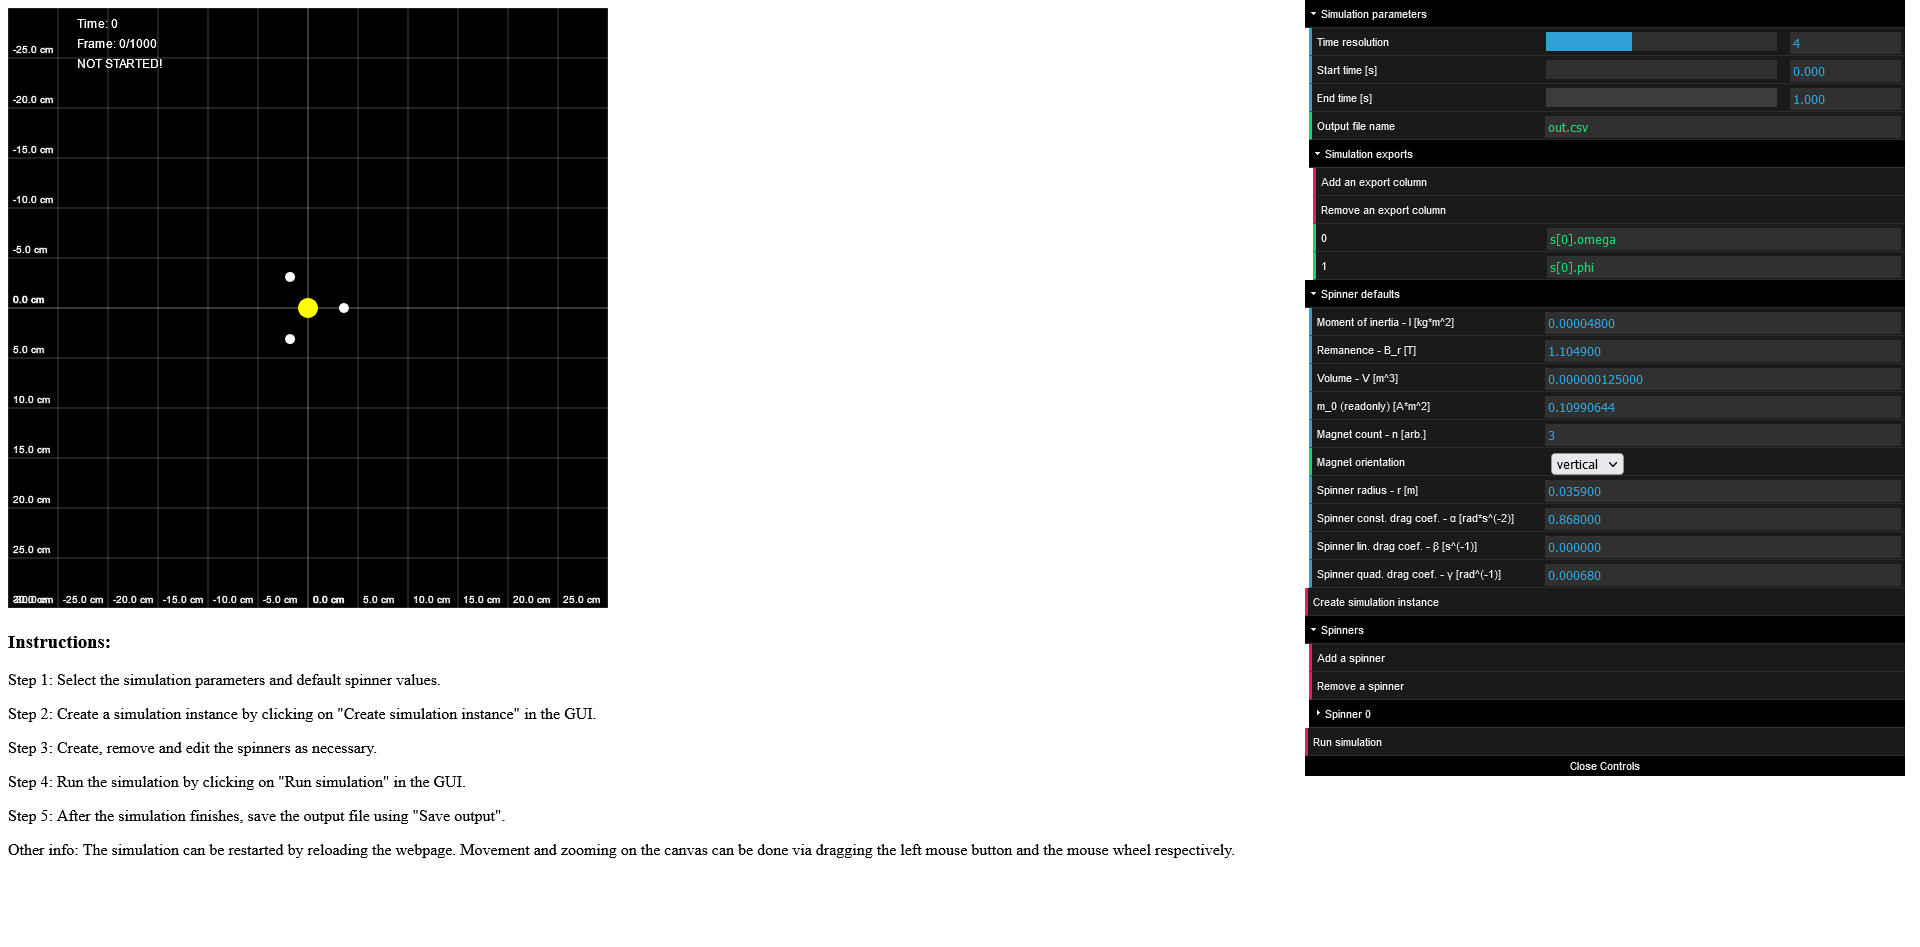
\includegraphics[width=0.9\textwidth]{screenshot_web_interface.png}
    \caption{Ukázka webového rozhraní}
    \label{fig:web_interface}
\end{figure}